\documentclass{article}
\usepackage{ijcai05}
\usepackage{times}
\usepackage{latexsym}
\usepackage{amsfonts}
\usepackage[pdftex]{graphicx}
\usepackage{algorithm}
\usepackage[noend]{algpseudocode}

\newtheorem{complexity}{Complexity}
\newtheorem{theorem}{Theorem}
\newtheorem{lemma}{Lemma}
\newtheorem{definition}{Definition}
\def\qed{\hfill \quad \vrule height4.17pt width4.17pt depth0pt} 
\newenvironment{proof}[1][Proof]{\noindent \textbf{#1:} }{\qed}
\newcommand{\maxflow}{\mathrm{maxflow(}n,m\mathrm{)}}
\newcommand{\ixtet}{I{\scriptsize X}T{\scriptsize E}T\hspace*{1mm}}

\title{New results on the resource-constrained project scheduling problem based on a pure constraint programming approach\\
- WORKING PAPER, PLEASE DO NOT DISTRIBUTE -}

%%New lower bounds results on discrete resources}

\author{Philippe Laborie \\ ILOG \\ 9, rue de Verdun, 94253 Gentilly
Cedex, France \\ plaborie@ilog.fr}

\begin{document}

\maketitle

\begin{abstract} 
This paper presents new   results on the  resource-constrained project
scheduling  problems (RCPSP) based  on a  very  simple complete search
procedure implemented   on  top  of classical  constraint  propagation
algorithms\footnote{Those algorithms  are all available in the current
release  of      ILOG   Scheduler  \cite{scheduler-60}.    See    {\tt
http://www.ilog.com}.}.  Using this  approach,  we were able  to close
15\%    of   the  previously open    problems    of the  PSPLIB
\cite{kolisch-sprecher-96} with 60,90 and  120 activities (93 problems
were closed) and improve more than 30\% of the previously best known lower
bounds on those problems (192 lower bounds were improved).
\end{abstract}

%% minimal critical sets \sep constraint propagation \sep Cumulative resources 

\section{Introduction}

The  resource constrained  project  scheduling problem  (RCPSP) can be
stated as follows:   a single project   consists  of a  number  of $n$
activities $\{A_1,...,A_n\}$ where each  activity has to be  processed
in order to complete  the project. The  activities are interrelated by
two kinds of constraints. First, precedence constraints force activity
$A_i$ not to  be started  before  all its immediate  predecessors have
been finished.   Second, performing  the activities requires resources
with limited  capacities. Altogether there  is a set of  $q$ resources
$\{ R_{1},...,R_{q}\}$. While being processed, activity $A_i$ requires
$q_{i,j}$  units  of resource  $R_j$ in  every   time  instant of  its
non-preemptable duration $p_i$.  Resource $R_j$ has a limited capacity
of $Q_j$ at  any point in  time. The parameters $p_i$,  $q_{i,j}$, and
$Q_j$ are  assumed to be nonnegative  and deterministic. The objective
of the  RCPSP is to find  precedence and  resource feasible completion
times  for  all activities such that  the  makespan of the  project is
minimized.

The decision variant  of the RCPSP, i.e.,  the  problem of determining
whether  there exists a  feasible project  of makespan  smaller than a
given deadline, is NP-hard  in the strong sense.  The  RCPSP is a very
popular  and frequently  studied  NP-hard optimization  problem and the
last  20   years  have  witnessed  a  tremendous improvement   of both
heuristic and exact solution  procedures (cf.  e.g. the recent surveys
given     in         Demeulemeester                and       Herroelen
\cite{demeulemeester-herroelen-02},    Hartmann     and        Kolisch
\cite{hartmann-kolisch-04},         Kolisch         and         Padman
\cite{kolisch-padman-01}).   The currently  best  lower bounds  on the
makespan  for the RCPSP   are based on  solving  linear programs using
adequate cutting planes \cite{brucker-knust-00,baptiste-demassey-04}.

In  this article, we  present  a pure constraint  programming approach
based on the  exploration of a complete search  tree to prove that the
project  cannot be achieved  within a given  deadline or to exhibit a
feasible project if one exists.  The search  procedure is based on the
detection and     resolution   of   {\em  minimal    critical    sets}
\cite{laborie-ghallab-95} at each node of the search. Minimal critical
sets are carefully  chosen using a  heuristics that tries  to minimize
the size of  the search tree. During  the search, a strong  constraint
propagation  is  enforced   using  classical   constraint  propagation
techniques such   as  {\em   time-tabling}, {\em edge-finding}, 
{\em precedence energy} and {\em balance} constraints.

Next section introduces the main notations used  in the article. Then,
section \ref{propagation}   recaps  the principle of   the  constraint
propagation  algorithms we   are  using.  Section   \ref{basic-search}
describes   our basic search  procedure  as well  as the heuristics to
select minimal critical sets. A first series of experimental results on
the instances of the PSPLIB using this basic search procedure is given
in section \ref{experiments-1} and   shows  that even such  a   simple
approach allows to close more  than 13\% of previously open  instances
and to improve about 30\% of best known  lower bounds within a 300s time-limit.   
The last section extends the basic   search procedure to  perform some  kind of
{\em self-adapting shaving} that still helps improving the results. 

\section{Model and Notations} \label{notations}

The resource constrained  project scheduling  problem (RCPSP)  can  be
formally stated as follows: Given

\begin{enumerate}

\item A set of $q$ resources $\{ R_{1},...,R_{q}\}$ with capacity $Q_{1},...,Q_{q}$.

\item A set of $n$ non-preemptable activities $\{ A_{1},...,A_{n}\}$ of
given   processing  time  $p_{1},...,p_{n}$. 

\item A network of precedence constraint between the activities modeled
as a directed acyclic graph G.

\item For each activity $A_{i}$ and each resource $R_{j}$, the amount
$q_{ij}$ of the resource required by  the activity over its execution.
If $q_{ij}>0$,  we will  denote $u=(A_{i},R_{j},q_{ij})$  the resource
requirement of activity   $A_{i}$  on  resource $R_{j}$ and     denote
$q(u)=q_{ij}$    and      $A(u)=A_{i}$.  $p(u)$ denotes the processing time of the activity of $u$. 
$s(u)$ (resp. $e(u)$) will 
denote the start (resp. end) time of the activity of $u$. $s_{min}(u)$, 
$s_{max}(u)$,  $e_{min}(u)$, $e_{max}(u)$ respectively denote the current 
minimal start time, maximal start time, minimal end time and maximal end 
time of the activity of $u$.  We    will    also    denote 
$U(R_{j})=\{(A_{i},R_{j},q_{ij})/q_{ij}>0\}$ the set of resource 
requirements on resource $R_{j}$.

\end{enumerate}

The goal of the RCPSP is to find a schedule meeting all the constraint
whose makespan (i.e. the time at which all activities are finished) is
minimal.

If   $\phi \subseteq  U(R_{j})$  is a  subset  of
resource   requirements  on   a   resource  $R_j$,  we   will   denote
$q(\phi)=\sum_{u \in \phi}{q(u)}$ the global resource consumption of 
activities in $\phi$.
 
\section{Constraint Propagation} \label{propagation}

The search procedure we will describe in  next section was implemented
on top of a  strong constraint propagation   scheme using most  of the
classical  algorithms available  in constraint-based scheduling. Those
algorithms are summarized below. We limit ourselves to the special case 
of discrete resources with constant resource requirements which is the 
case of the instances of the PSPLIB\footnote{The propagation algorithms 
presented in this section work in more general cases where the quantity 
of resource required is also a decision variable. Furthermore, the 
timetabling and the balance constraint also work on the more general 
case of reservoir resources where the resource can be independently 
consumed or produced by activities.}. All these algorithms are available 
in the current release of ILOG Scheduler \cite{scheduler-60}.

\subsection{Timetabling}

The first  propagation technique, known as  {\bf timetabling}, relies on the
computation for every date  $t$ of the minimal  resource usage at this
date by the current activities in  the schedule \cite{lepape-94}. This
aggregated demand profile  is maintained during  the search. It allows
us to restrict the domains of the start and end times of activities by
removing the dates that  would necessarily lead to an over-consumption
of the resource.

Suppose  a resource  requirement    $u=(A,R,q)$ on a  given   discrete
resource $R$ that is  such that $s_{max}(u) <  e_{min}(u)$, then
we know surely  that $A$ will at least  execute over the time interval
$[s_{max}(u),  e_{min}(u))$.  Thus, it  will surely  require $q$
units of resource $R$ on this time interval.  For each resource $R$, a
curve $C_R(t)$ is maintained that aggregates all these demands:

\[C_R(t) = \sum_{ \{u \in U(R)/ s_{max}(u) \le t < e_{min}(u)\}}
\hspace{-15mm} q(u) \] 

It is  clear that if there  exists  a date  $t$  such that $C_R(t)$ is
strictly  greater than $Q$, the  maximal capacity of the resource, the
current  schedule  cannot  lead to   a solution and   the search  must
backtrack.     Furthermore, if  there   exists  a resource requirement
$u=(A,R,q)$ and a date $t_0$ such that:

\begin{enumerate}
\item $e_{min}(u) \le t_0 < e_{max}(u)$ and;
\item $\forall t \in [t_0, e_{max}(u)), C_R(t) + q > Q$
\end{enumerate} 

then, the activity of $u$ cannot end after  date  $t_0$.  It would otherwise
over-consume the resource.    Indeed, remember that,  as $e_{min}(u)
\le t_0$, $A$ is  never taken into account in  the aggregation on  the
time interval $[t_0  , e_{max}(u)$).   Thus,  $t_0$ is  a new  valid
upper bound for $e(u)$.

Similar reasoning can be applied to find new lower bounds on the start
time  of activities.

\subsection{Edge-Finding.}          

Let $\phi \subset U(R)$ a subset of resource requirements on a resource $R$ of capacity $Q$ and $u \in U(R)\setminus \phi$. Let's denote:
\begin{itemize}
\item $s_{min}(\phi)=\min_{x \in \phi}{s_{min}(x)}$, 
\item $e_{min}(\phi)=\min_{x \in \phi}{e_{min}(x)}$, 
\item $e_{max}(\phi)=\max_{x \in \phi}{e_{max}(x)}$, 
\item $w(\phi)=\sum_{x\in \phi}{p(x).q(x)}$. 
\end{itemize}

The edge-finding algorithms \cite{nuijten-94} performs the three following deduction rules:

{\bf Rule 1.} if $Q.(e_{max}(\phi) - s_{min}(\phi \cup \{u\})) < w(\phi \cup \{u\})$, then $u$ must finish after all the activities in $\phi$.

{\bf Rule 2.} if $s_{min}(\phi) < s_{min}(u) < e_{min}(\phi)$ and $Q.(e_{max}(\phi) - s_{min}(\phi)) < w(\phi) + q(u).(min(e_{max}(\phi), e_{min}(u))-s_{min}(\phi))$, then at least one activity $x$ in $\phi$ must precede $u$ as otherwise, $u$ would start between $s_{min}(\phi)$ and $e_{min}(\phi)$ and there would not be enough energy to execute $\phi \cup \{u\}$ between $s_{min}(\phi)$ and $e_{max}(\phi)$.
	
{\bf Rule 3.} if $s_{min}(u) < s_{min}(\phi) < e_{min}(u)$ and $Q.(e_{max}(\phi) - s_{min}(\phi)) < w(\phi)+ q(u).(e_{min}(u)-s_{min}(\phi))$, then  $u$ must finish after all the activities in $\phi$.

The three rules above allows to update the minimal start or end times of 
activities and symmetrical rules allow to update the maximal start and end times.

\subsection{Precedence Graph}

The {\bf precedence graph} is the basic structure used by the two propagation 
algorithms outlined in section \ref{energyprecedence} (energy precedence) and 
\ref{balance} (balance constraint).

\subsubsection{Definitions} 
A {\bf resource  event} $x$  on a  given resource $R$  is a time-point
variable at which the availability of  the resource changes because of
an activity.  A  resource event corresponds to  the start or end point
of an activity. Let:
\begin{itemize}
\item $t(x)$ denote the time-point variable of event $x$. $t_{min}(x)$
      and  $t_{max}(x)$ will respectively  denote  the current minimal
      and maximal value in the domain of $t(x)$.
\item $q(x)$ denote the  relative change of resource  availability due
      to event  $x$ with the convention  that $q>0$ denotes a resource
      production and   $q<0$ a resource  consumption.
\end{itemize}  

For the RCPSP, a resource requirement $u=(A,R,q)$ is represented by two events 
on resource $R$: an event at the start time of the activity that consumes $q$ 
units of the resource $(s(u),-q)$ and an event at the end time of the activity that 
produces (releases) $q$ units of the resource $(e(u),+q)$.

A {\bf precedence   graph}  on a resource    $R$ is a directed   graph
$G_R=(V,E_{\le},E_{<})$ where $E_{<} \subset E_{\le}$ and:
\begin{itemize}
\item $V$ is the set of resource events on $R$ 
\item $E_{\le}  ={(x,y)}$ is the set   of precedence relations between
      events of the form $t(x) \le t(y)$.
\item $E_{<} ={(x,y)}$   is the  set of precedence   relations between
      events of the form $t(x) < t(y)$.
\end{itemize}

The precedence graph on  a  resource is  designed  to collect all  the
precedence  information    between  events  on     the resource. These
precedence information may come from: (1)  temporal constraints in the
initial statement  of  the problem,  (3) search   decisions
(e.g. ordering  decisions    on
resources)  or (4) may  have been discovered by propagation algorithms
(e.g. edge-finding, balance constraint, etc.) or simply because $t_{max}(x) \le
t_{min}(y)$. When new events or new precedence relations are inserted,
the   precedence    graph  incrementally  maintains    its  transitive
closure. This leads to a worst-case complexity of $O(n^2)$ to maintain
the precedence graph. The precedence relations in the precedence graph
as well as  the  initial  temporal  constraints are propagated  by  an
arc-consistency algorithm. Given an event  $x$  in a precedence  graph
and assuming the  transitive closure has been  computed, we define the
following subsets of events:
\begin{itemize}
\item $S(x)$ is  the set of events simultaneous  with  $x$ that is the
      events $y$ such that $(x,y) \in E_{\le}$ and $(y,x) \in E_{\le}$
\item $B(x)$ is the set  of events before $x$  that is the events  $y$
      such that $(y,x) \in E_{<}$
\item $BS(x)$ is  the set  of events  before or  simultaneous with $x$
      that  is the events $y$  such that $(y,x)  \in E_{\le}$ , $(y,x)
      \notin E_{<}$ and $(x,y)\notin E_{\le}$
\item $A(x)$ is the  set of events after   $x$ that is the events  $y$
      such that $(x,y)\in E_{<}$
\item $AS(x)$ is the set of events after or simultaneous with $x$ that
      is the events  $y$ such  that that  $(x,y)\in  E_{\le}$ , $(x,y)
      \notin E_{<}$ and $(y,x)\notin E_{\le}$
\item $U(x)$ is the set of events unranked with respect to $x$ that is
      the events $y$  such that $(y,x)\notin E_{\le}$ and $(x,y)\notin
      E_{\le}$
\end{itemize}

Note that $\{S(x), B(x), BS(x), A(x),  AS(x),U(x)\}$ is a partition of
$V$.  

\subsubsection{Implementation and Complexity}

As we will see in next  section, our propagation algorithms often need
to query  the precedence graph   about  the relative position  of  two
events on a  resource  so this  information needs to  be accessible in
$O(1)$ on  our structure. It  explains  why we  chose to implement the
precedence  graph as a matrix   that  stores the relative position  of
every pair of events. Furthermore, on our structure, the complexity of
traversing any  subset of events (e.g. $B(x)$  or $U(x)$)  is equal to
the  size of this subset. 

\subsection{Energy Precedence Constraint} \label{energyprecedence}

The    {\bf  energy precedence constraint} \cite{laborie-03} is     defined on discrete
resources only.   If $x$ is a  resource event and $\varphi \subset U(R)$
is a  subset of resource requirements  that, given the current precedence graph,
are constrained to execute before  $x$, then the resource  must  provide enough energy to execute
all resource requirements in $\varphi$ between  the earliest start times
of activities of $\varphi$ and $t(x)$. More formally:

\[t_{min}(x) \ge \min_{u \in \varphi} (s_{min}(u)) + \sum_{u\in \varphi}(q(u)p(u)) / Q \]

A very simple example of the  propagation performed by this constraint
is given in Figure \ref{fig:figure3}. If we suppose that the maximal capacity
of the resource is $4$  and all activities must  start after
time $0$, then by considering  $\varphi=\{u_1, u_2, u_3, u_4\}$, we see
that          event  $x$   cannot         be  executed    before  time
$[0]+[(2 \cdot 10)+(2 \cdot 8)+(2 \cdot 8)+(2 \cdot 2)]/4 = 14$. Of course, a symmetrical rule
can be used  to  find  an upper  bound  on $t(x)$  by considering  the
subsets $\varphi$  of  resource  constraints  that must  execute  after
$x$. 

\begin{figure}
	\centering
		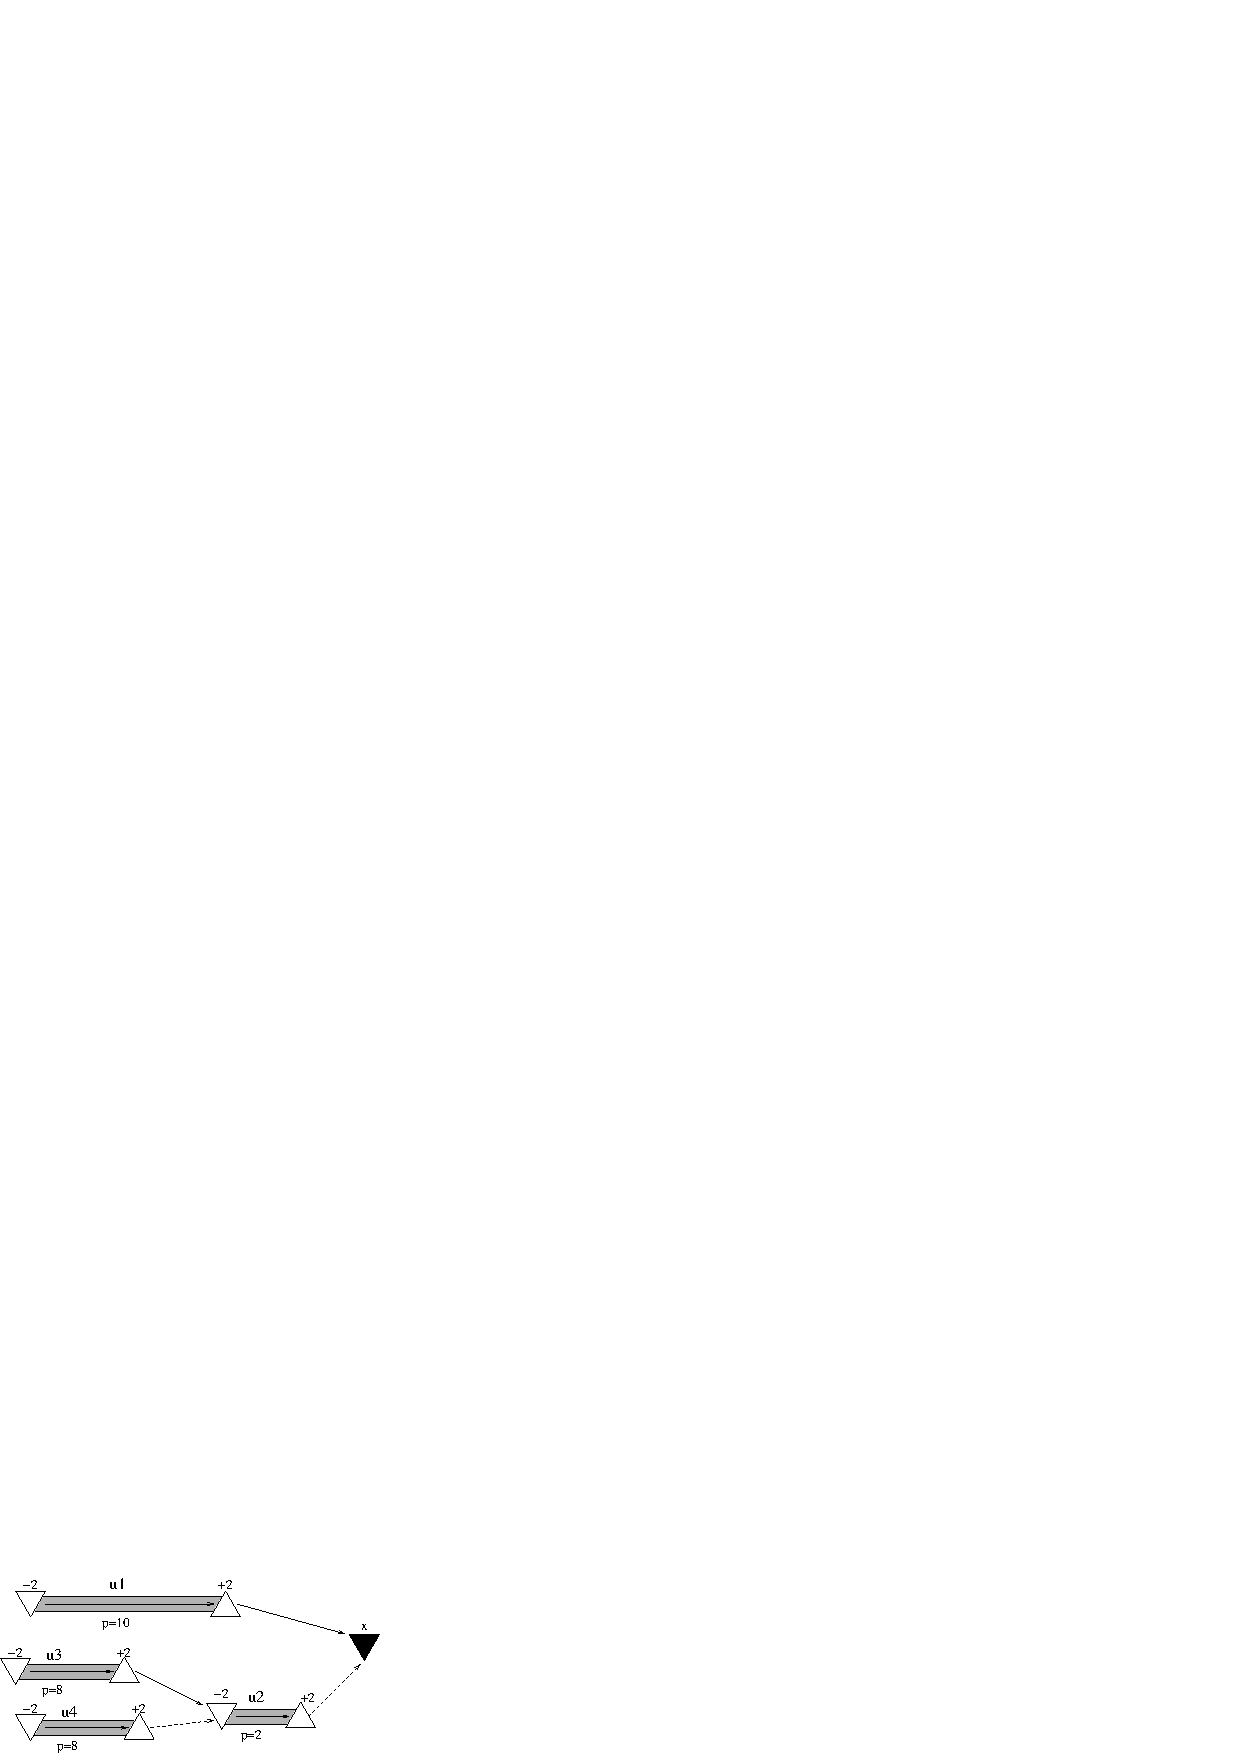
\includegraphics{figures/figure3.pdf}
  \caption{Energy precedence constraint}
	\label{fig:figure3}
\end{figure}

The propagation of the energy precedence constraint can be
performed for all the events $x$ on a resource and for all the subsets
$\varphi$ with  a total worst-case  time complexity of $O(n (p+log(n))$
where $n$ is  the number  of the events  on  the resource and $p$  the
maximal number  of predecessors of a  given  event in the  graph ($p <
n$). 

\subsection{Balance Constraint}\label{balance}

On a discrete resource, the {\bf balance constraint} \cite{laborie-03} can be defined as follows. 
The basic idea  of the algorithm is to compute, for each event $x$ 
in the precedence graph, a lower bound on the resource usage at the time-point $x$. 
In what follows, we assume $x$ is a consumption event corresponding 
to the start time of a resource requirement, a symmetrical reasoning 
can be applied to a production event.

Using the precedence graph we can compute  a lower bound  on the resource utilization
at   date  $t(x)+\epsilon$ just after $x$ assuming that all the resource requirements 
that do not necessarily overlap $x$ will not overlap it:

\begin{eqnarray*}
L_{min}(x) = \sum_{u / s(u) \in B(x) \cup BS(x) \cup S(x), e(u) \in A(x)} q(u) 
\end{eqnarray*}

Applying this  formula   to event  $x$ in  Figure   \ref{figure4} 
leads to $L_{min}(x)=q(u_3)+q(u_1)=3$. 

Given this bound, the balance constraint is able  to discover three types  of information:  {\bf dead
ends}, new  bounds for  {\bf time variables} and new {\bf precedence relations}. 

\begin{figure}
	\centering
		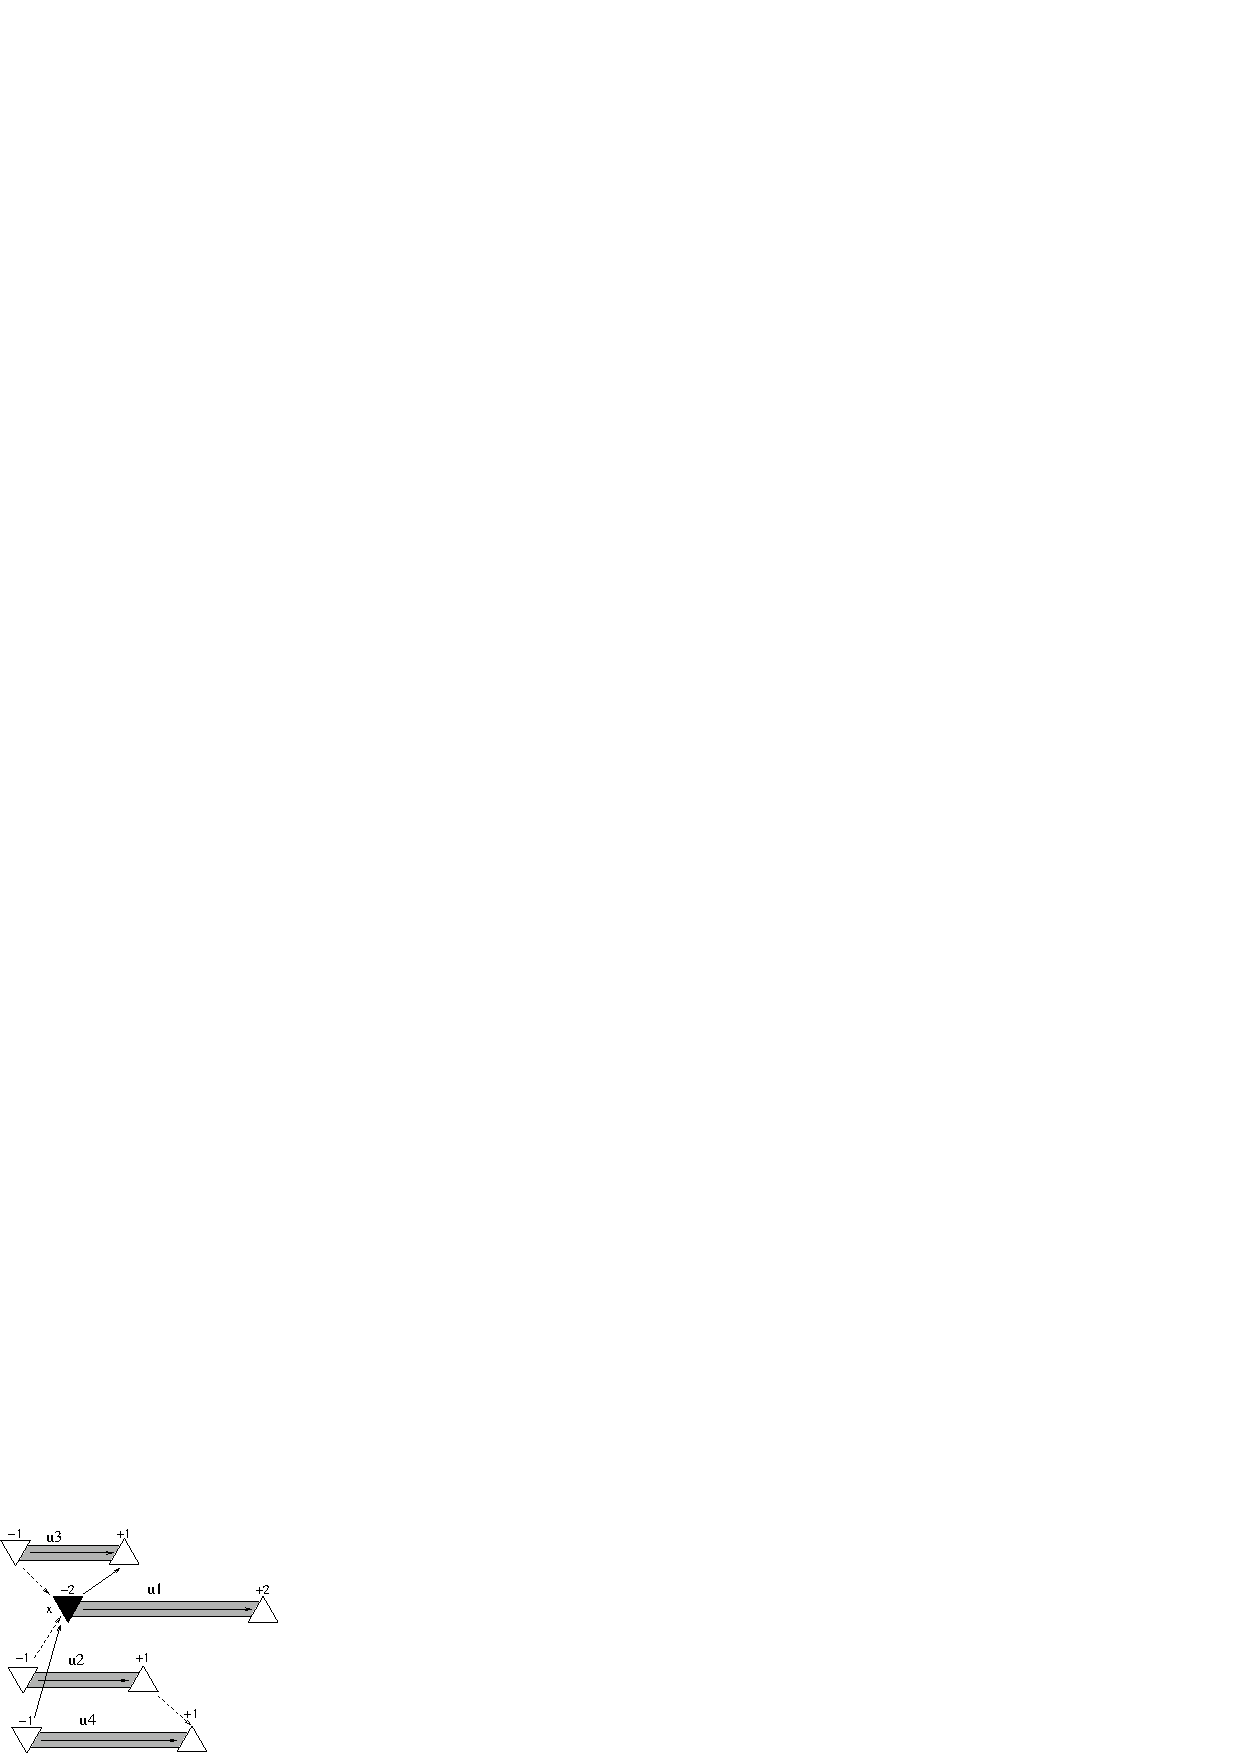
\includegraphics{figures/figure4.pdf}
	\caption{Balance constraint}
	\label{figure4}
\end{figure}

\subsubsection{Discovering dead ends.} 

Whenever $L_{min}(x)>Q(R)$, we know that the  resource will  surely  be over-consumed just
after event $x$ so the search has reached a dead end.

\subsubsection{Discovering new bounds on time variables.} 

If $L_{min}(x) \leq Q(R)$, $\Delta(x)=Q-L_{min}(x)$ represents a slack of capacity that must not 
be exceeded by all the resource requirements that, currently, do not necessarily overlap $x$ 
but could overlap it. Let:
\[P(x)=\{e(u)/s(u)\in B(x) \cup BS(x) \cup S(x), e(u) \notin A(x)\}\]

We suppose the events $(y_1,\cdots,y_i,\cdots,y_p)$ in $P(x)$ are ordered
by  decreasing minimal  time $t_{min}(y)$. Let   $k$ be  the index  in
$[1,p]$ such that:

\begin{eqnarray*}
\sum_{i=1}^{k-1}q(y_i) \le \Delta(x) < \sum_{i=1}^{k}q(y_i)
\end{eqnarray*}

If event $x$ is executed at a date $t(x) < t_{min}(y_k)$, not enough
producers will be  able to  execute strictly before   $x$ in order  to
ensure the resource is not overconsumed just after $x$ as in this case, 
the consumed quantity will be at least $L_{min}(x)+\sum_{i=1}^{k}q(y_i)>Q(R)$.  Thus, $t_{min}(y_k)$ is a
valid  lower  bound of $t(x)$. 

In   Figure \ref{figure4} if the maximal capacity of the resource is $4$, 
thus $\Delta(x)=1$,  this propagation  will deduce  that $t(x)$
must  be greater than the   minimum between the earliest end
time of $u_2$ and the earliest end time of $u_4$.

\subsubsection{Discovering new precedence  relations.} There are cases
where we can  perform  an  even  stronger propagation. Suppose   there
exists a production event $y$ in $P(x)$ such that:

\begin{eqnarray*}
\sum_{z \in P(x) \cap (A(y) \cup AS(y) \cup S(y))} q(z) > \Delta(x)
\end{eqnarray*}

Then, if we had  $t(x) < t(y)$, we would see  that again there is  no
way to avoid a resource over-consumption as it would consume at least:

\begin{eqnarray*}
L_{min}(x)+\sum_{z \in P(x) \cap (A(y) \cup AS(y) \cup S(y))} q(z) > Q
\end{eqnarray*}

Thus,  we can deduce the necessary
precedence relation:  $t(y) \leq t(x)$.  For example  in Figure \ref{figure4},
the balance algorithm  would  discover that  $x$ needs to  be executed
after the  end of $u_2$. 

Like for  timetabling   approaches, one  can  show that  the
balance algorithm is  {\bf sound}, that is,  it will detect a dead end
on any fully  instantiated  schedule   that violates the  
resource  maximal capacity.   Note also that, according
to the concepts introduced in \cite{laborie-ghallab-95}, the balance constraint
can be  seen as an algorithm that  implicitly  detects and solves some
deterministic  MCSs on the resource while avoiding the combinatorial
explosion of enumerating  these  MCSs.  The balance algorithm   can be
executed for all the events $x$ with a global worst-case complexity in
$O(n^2)$ if the propagation that discovers new precedence relations is
not turned on, in $O(n^3)$ for a  full propagation. In practice, there
are many  ways to  shortcut  this worst  case  and  in particular,  we
noticed that the   algorithmic   cost of  the   extra-propagation that
discovers new    precedence    relations  was  negligible.   In    our
implementation,    at each node  of   the   search,  the full  balance
constraint is executed until a fix point is reached.

\section{Search}
\label{basic-search}

\subsection{Branching Scheme}

The branching scheme relies on the notion of minimal critical sets and
their resolvers as  introduced in \cite{laborie-ghallab-95}. A minimal
critical set (MCS) is  a minimal set  (in the  sense of   set inclusion) of
resource requirements that could be executed simultaneously and could 
over-consume the resource.

\begin{definition}[Minimal critical set]  
A minimal critical set on  a  resource $R_{j}$  is a subset $\phi\subseteq U(R_{j}),$ such that:
\begin{enumerate}
\item $Q_{j}<q(\phi)$
\item $\forall\varphi\subset\phi,\varphi\neq\phi$,$q(\varphi)\leq Q_{j}$
\item $\bigwedge_{(u,v)\in\phi\times\phi}s(u)<e(v)$
is consistent with the current temporal constraints
\end{enumerate}
\end{definition}

Informally,   the  different ways to  resolve  a  minimal critical set
consist   in posting a  precedence  constraint between any  two of its
activities.

\begin{definition}[Resolvers of a minimal critical set] 
If $\phi\subseteq   U(R_{j})$ is a MCS,   we call
resolvers   of $\phi$  the   disjunctive set  of  temporal constraints
$Res(\phi)=\{e(u)\leq s(v)\}_{(u,v)\in\phi\times\phi,u\neq
v}$.
\end{definition}

As  described  in  \cite{laborie-ghallab-95},   the set  of  resolvers
$Res(\phi)$ of a MCS  $\phi$ can be minimized  so  as to remove  those
resolvers  $\rho\in Res(\phi)$ that  are so that  there exists another
resolver $\rho'\in Res(\phi)$ such  that $\rho\Rightarrow\rho'$ on the
current temporal  network.  Indeed, in  such case, the resolver $\rho$
is redundant.  Such  a  minimization procedures  can be   achieved  in
$O(k^{3})$ if $k$ is the  size of the  MCS using the naive algorithm 
Alg \ref{minimize}. In what follows, we assume
that the set of resolvers of a MCS has been minimized.

\begin{algorithm}
\caption{Resolver Minimization algorithm} \label{minimize}
\begin{algorithmic}[1]

\Procedure{MINIMIZE\_RESOLVERS}{$\phi$}
\State $Res(\phi) \leftarrow \emptyset$
\ForAll{$u$ {\bf in} $\phi$}
\ForAll{$v$ {\bf in} $\phi$ {\bf such that} $u \neq v$}
\State $uv \leftarrow$ TRUE
\ForAll{$w$ {\bf in} $\phi$}
\If{$s(v) \leq s(w)$ {\bf or} $e(w) \leq e(u)$ }
\State $uv \leftarrow$ FALSE
\State {\bf break}
\EndIf
\EndFor
\If{$uv$}
\State $Res(\phi)\leftarrow Res(\phi) \oplus(e(u) \leq s(v))$
\EndIf
\EndFor
\EndFor
\State {\bf return} $Res(\phi)$
\EndProcedure
\end{algorithmic}
\end{algorithm}

\subsection{Heuristics}\label{heuristics}

Let $x$  and $y$ be  two time-points (start  or end of an activity) in
the schedule. As all the  resolvers consist of temporal constraints of
the form $x\leq y$, we are interested in  the size of the search space
after posting  such a precedence constraint. To  estimate the ratio of
the  search  space    that is  preserved  when     adding a precedence
constraint,  we  use   the complementary   of   the commitment measure
introduced in \cite{laborie-03}.

Let  $x$ and $y$  be two  time-points with  respective lower and upper
bound  for time value:  $x_{min},x_{max},y_{min},y_{max}$. The size of
the search  space is estimated by  the cartesian product of the domain
of  the  two   variables,  that  is,  the    area  of the    rectangle
$x_{min},x_{max},y_{min},y_{max}$.  The  size of the search space that
is preserved when adding the constraint $x\leq y$ is  the part of that
rectangle above the line $x=y$ as illustrated in Fig \ref{fig1}.

\begin{figure}
\centerline{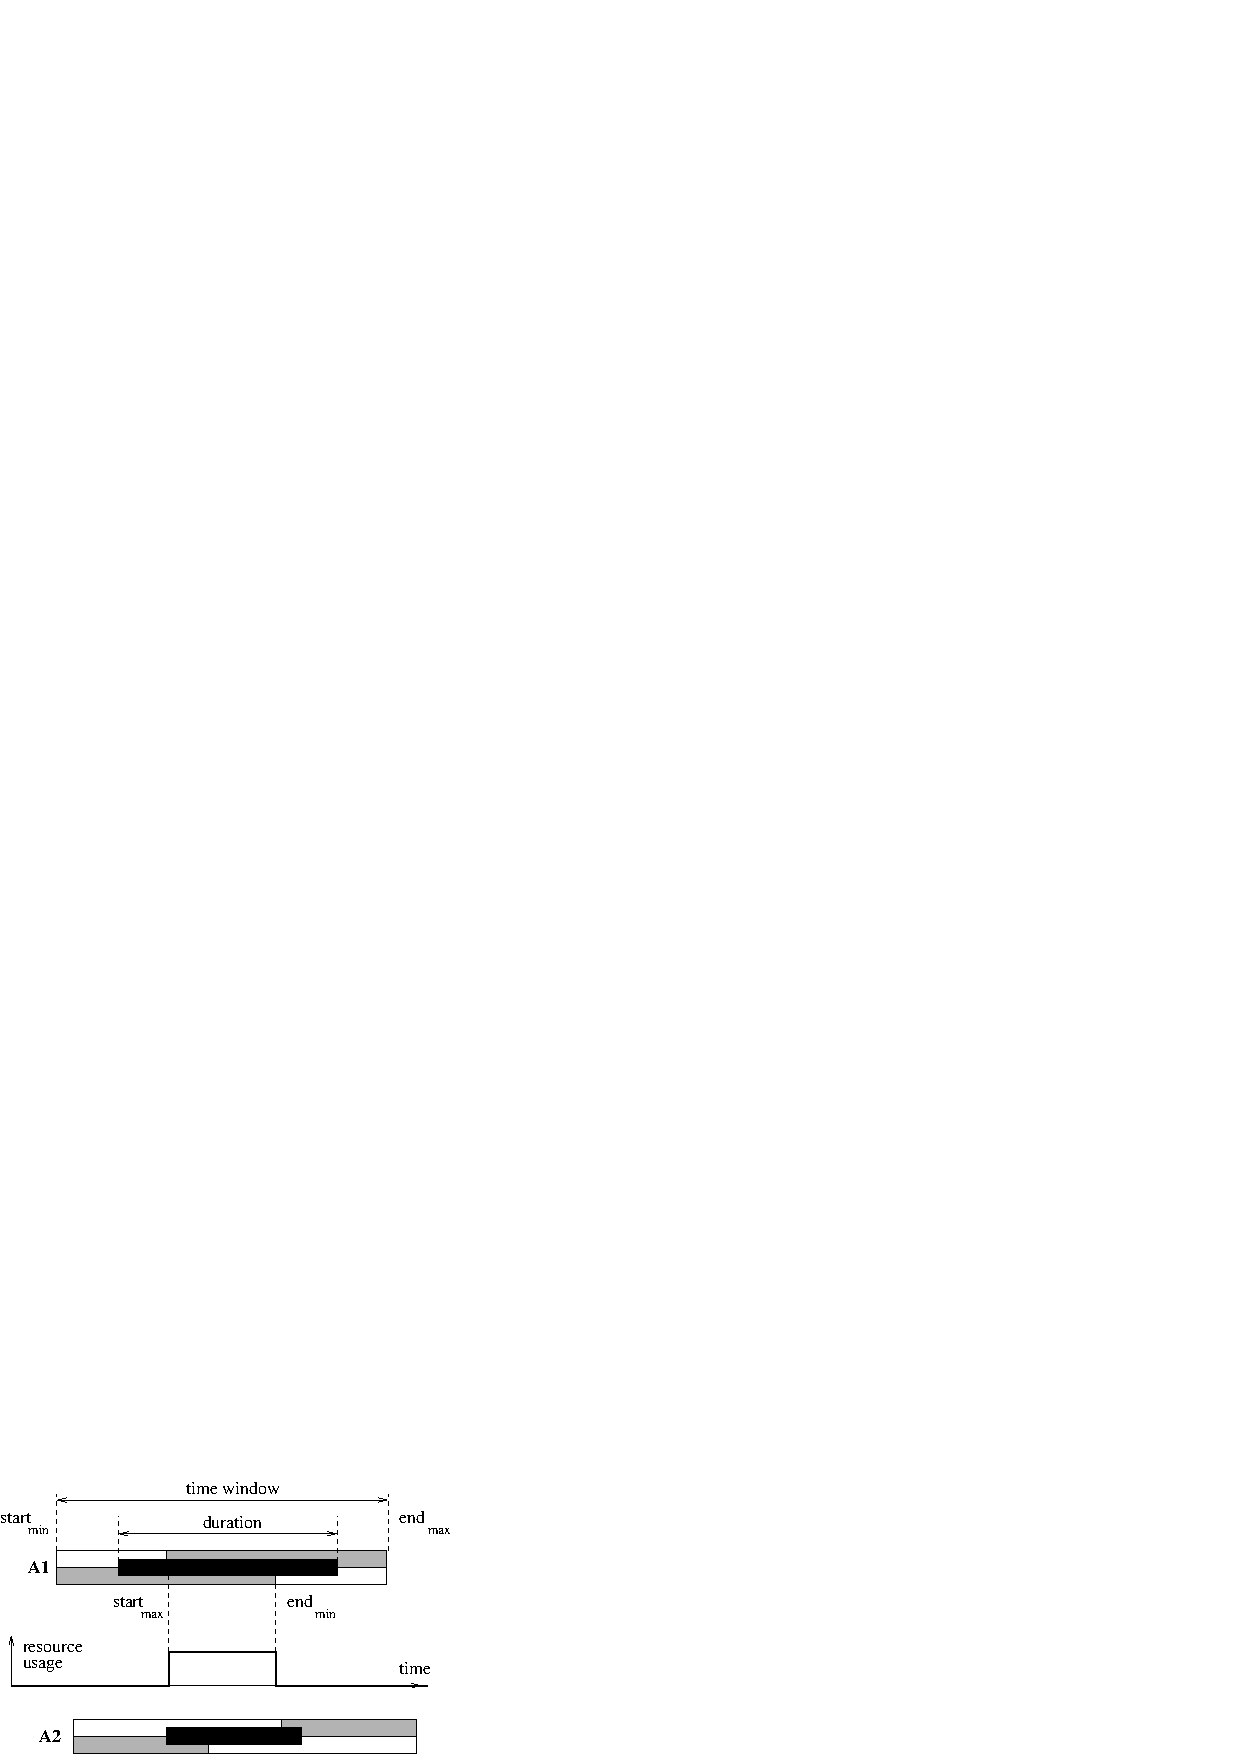
\includegraphics[width=10pc]{figures/fig1.pdf}}
\caption{Preserved search space when adding $x\leq y$}
\label{fig1}
\end{figure}

The ratio of the search space that is preserved can thus be estimated
as follows. Let:
\[A=(y_{max}-y{}_{min}+1)(x_{max}-x_{min}+1)\]
\[B=(y_{max}-x_{min}+1)^{2}\]
\[C_{min}=max(0, y_{min}-x_{min})^{2}\]
\[C_{max}=max(0, y_{max}-x_{max})^{2}\]

The ratio is then equal to: 

\[preserved(x\leq y)=\frac{B- C_{min} - C_{max}}{2A}\]

If $\omega$ is the  size of the search  space below the current search
node, the size of the search space after posting a temporal constraint
$x\leq y$ can be estimated by $\omega.preserved(x\leq y)$.

If $\phi$ is the  MCS that is selected to  be resolved at the  current
search node, the size  of the search  space below the current node can
be estimated as the sum of the sizes of the  search space below each child
node,               that             is:        $\omega.\sum_{\rho\in
Res(\phi)}preserved(\rho)$. Thus,    $preserved(\phi)=\sum_{\rho\in
Res(\phi)}preserved(\rho)$  estimates  the search  space ratio that is
preserved when choosing $\phi$ as the next MCS to solve \footnote{Note
that  this is of  course only a rough estimate  and in particular, the
estimated ratio  $preserved(\phi)$  can  be greater  than  1.   }. Our
heuristics  simply   chooses  to  resolve  next  the  MCS $\phi$  that
minimizes $preserved(\phi)$.   Once  this MCS  has  been selected, the
algorithm branches on  the different resolvers  $\rho\in Res(\phi)$ by
decreasing order of $preserved(\rho)$.

\subsection{MCS Selection algorithm}

The  approach  has  been implemented   on top of   ILOG Scheduler  6.0
\cite{scheduler-60} using the {\em timetable}, {\em disjunctive}, {\em
edge-finder},    {\em   precedence   energy}    and    {\em   balance}
constraints described in section \ref{propagation}. At each search node, the MCS selection procedure explores
a tree of  partial MCS where the  current  MCS is extended  adding one
resource requirement  in the child of  a given node.  By definition of
$preserved(\phi)$,    it  is clear  that  $\phi'\subset\phi\Rightarrow
preserved(\phi')\leq  preserved(\phi)$.    Thus, if $\phi^{*}$  is the
best MCS found so far, once a partial MCS $\phi$ has been reached such
that $preserved(\phi^{*})\leq preserved(\phi)$, the subtree of the MCS
selection tree  rooted at $\phi$ can  be abandoned.  

The algorithm for  selecting and branching on a  MCS is more precisely
described  in Alg \ref{selectmcs} using the following  notations:  $id(u)$ is a  unique
index associated with resource   requirement $u$ used to  break  ties.
$Unranked(u)$  represents   all the  resource  requirements $v$ that  can
possibly overlap $u$ given the current temporal constraints, and that are 
so that $q(v)<q(u)$ or $q(v)=q(u)$ and $id(v)<id(u)$. $\phi$ is
the current (partial) MCS.   A (partial) MCS  is represented by a list
of resource   requirements: $\phi=(u_1,...,u_k)$.  We  denote  $u_k  =
Last(\phi)$ and define the operator  $\oplus$ as follows: $\phi \oplus
u=(u_1,...,u_k,u)$.   $q=q(\phi)$  is the consumption   of the current
(partial)  MCS; $p=preserved(\phi)$ is the   preserved search space so
far in the current (partial) MCS; $\phi^*$ is  the best MCS so far and
$p^*=preserved(\phi^*)$ is the preserved  search space of the best MCS
so far.

The  procedure at line \ref{selectmcs0}  calls  the  MCS  rating and
selection process on each resources. At line    \ref{selectmcs1} the 
procedure to rate and select MCSs for a given resource first sorts the relevant sets of
requirements  $v$ at  lines \ref{sort1} and \ref{sort2}  by decreasing order of
$q(v$), using $id(v)$ to break ties in order to ensure that each MCS  is scanned only
once,  starting with the  smallest MCSs, that  is, the ones containing
the most greedy requirements. The procedure at line \ref{unranked} returns TRUE if and only if a given
requirement $u$ can possibly overlap all the requirements of a partial
MCS given the current temporal  constraints. This is done by  querying
the precedence graph. The procedure at line \ref{deltapreserved}  computes  the incremental
increase of preserved space due to  the insertion of a new requirement
$u$ in  the current  MCS $\phi$.   The  value of $preserved$  has been
described in section \ref{heuristics}. The main recursive function for selecting MCSs is described at line \ref{recselectmcs}. 

\begin{algorithm}
\caption{MCS Selection algorithm}\label{selectmcs}
\begin{algorithmic}[1]

\Procedure{SELECT\_MCS}{}\label{selectmcs0}
\State $p^* \leftarrow +\infty$
\For{$j$ $\leftarrow$ $1$ {\bf to} $q$}
\State SELECT\_MCS($R_j$)
\EndFor
\State {\bf return} $\phi^*$
\EndProcedure
\Statex

\Procedure{SELECT\_MCS}{$R$}\label{selectmcs1}
\State Sort $U(R)$ \label{sort1}
\ForAll{$u$ {\bf in} $U(R)$}
\State Sort $Unranked(u)$ \label{sort2}
\EndFor
\For{$u$ {\bf in} $U(R)$}
\State RSELECT\_MCS($R$,$(u)$,$q(u)$,$0$)
\EndFor
\EndProcedure
\Statex

\Procedure{IS\_UNRANKED}{$u$,$\phi$} \label{unranked}
\ForAll{$v$ {\bf in} $\phi$}
\If{$u \prec v$ {\bf or} $v \prec u$}
\State {\bf return} FALSE
\EndIf
\EndFor
\State {\bf return} TRUE
\EndProcedure
\Statex

\Procedure{DELTA\_PRESERVED}{$u$,$\phi$}\label{deltapreserved}
\State $dp$ $\leftarrow$ $0$
\ForAll{$v$ {\bf in} $\phi$}
\State $dp$ $\leftarrow$ $dp$ + preserved($u$,$v$) + preserved($v$,$u$)
\EndFor
\State {\bf return} $dp$
\EndProcedure
\Statex

\Procedure{RSELECT\_MCS}{$R$,$\phi$,$q$,$p$}\label{recselectmcs}
\If{$q>Q(R)$} \Comment{$\phi$ is a MCS}
\If{$p<p^*$} \Comment{$\phi$ is the best MCS so far}
\State $p^*$ $\leftarrow$ $p$
\State $\phi^*$ $\leftarrow$ $\phi$
\EndIf
\Else \Comment{$\phi$ needs to be extended}
\State $u$ $\leftarrow$ Last($\phi$)
\ForAll{$v$ {\bf in} Unranked($u$)}
\If{IS\_UNRANKED($v$,$\phi$)}
\State $dp$ $\leftarrow$ DELTA\_PRESERVED($v$,$\phi$)
\State RSELECT\_MCS($R$,$\phi \oplus v$,$q+q(v)$,$p+dp$)
\EndIf
\EndFor
\EndIf
\EndProcedure
\end{algorithmic}
\end{algorithm}

The best MCS $\phi^{*}$ that  has been scanned  by the above procedure
is selected as the one  to be solved  at the current search node. This
MCS is minimized and the search explores all of its resolvers $\rho\in
Res(\phi^{*})$ in  the    child   nodes   by   decreasing   order   of
$preserved(\rho)$.

\section{Experimental Results}
\label{experiments-1}

We evaluated the approach described above 
on the instances of the PSPLIB\cite{kolisch-sprecher-96} with 60, 90 and 
120 activities (resp. sets J60, J90, J120). For each instance, we solve 
the feasibility problem of finding a schedule with a makespan lower than $T$, 
starting with a valid lower bound for $T$\footnote{For instance the lower-bound of the PERT of temporal constraints} and incrementing $T$ until the problem is shown to be feasible (in this case, 
$T$ is the optimal makespan) or a until a given time limit for solving the problem with makespan $T$ is exceeded (in this case, $T$ is a valid lower-bound). For this experiment, we take a time limit of $300s$ on a Dell Latitude D600 laptop, 1.4 GHz. The approach was implemented on top of ILOG Scheduler 6.0.

The previous best lower and upper bounds we compare with are the ones reported in the PSPLIB 
together with the recent improvements on the J60 instances reported in \cite{baptiste-demassey-04}.
 
The results are summarized on Table \ref{tab:Results1} with the following columns:
\begin{description}
\item[\#O]: number of instances previously open
\item[\#I]: number of improved lower bounds (\% of \#O)
\item[AGR]: average gap (distance from the lower to the upper bound) reduction when a bound is improved
%\item[R]: ratio of the number of instances where the algorithms wins over the best known LB divided by the number of instances the algorithm looses
\item[\#C]: number of closed instances (\% of \#O)
\end{description}

\begin{table}
	\centering
		\begin{tabular}{|l|l|ll|l|ll|} \hline
			Inst. & \#O   & \#I &(\%I)    & AGR    & \#C &(\%C)   \\ \hline \hline
			J60		& 99		& 39  &(39.8\%) & 17.0\% & 21  &(21.2\%) \\ \hline
			J90		& 129		& 51  &(39.5\%) & 18.1\% & 26  &(20.2\%) \\ \hline
			J120	& 392		& 88  &(22.4\%) & 7.6\%  & 38  &(9.7\%) \\ \hline
			ALL   & 620   & 178 &(28.7\%) & 10.8\% & 85  &(13.7\%) \\ \hline
		\end{tabular}
	\caption{Results with a time-limit of 300s}
	\label{tab:Results1}
\end{table}

Out of the $620$ previously open instances, we are able to improve $178$ lower-bounds with 
an average gap reduction of $10.8\%$ and to close $85$ instances. 

%Another interesting result 
%is the robustness of the approach: on all the 1560 instances of the PSPLIB (480 for J60 
%and J90, 600 for J120), our algorithm improves the lower bound of 224 instances (the 
%cumulated improvement is equal to 634 time units) and is worse than the current best 
%known lower bound on 177 instances only (for a cumulated gap of 573 time units). 
%These figures show that our approach performs in average better than the conjunction 
%of all the previously reported techniques on the lower-bounds of the PSPLIB.


\section{Self-adapting shaving}
\label{shaving}

\subsection{Principles}

Shaving techniques \cite{torres-lopez-00} are all based on the following principle: 
if adding a constraint $C$ in the current node of the search leads to a failure of 
the propagation, then, constraint $\neg C$ can be inferred. Due to the cost of propagating 
a constraint $C$ and the potential number of constraints $C$ to try to shave on, 
shaving techniques are in general computationally expensive.  

We implemented the following shaving technique based on MCSs. If a MCS $\varphi$ 
with resolvers $Res(\varphi)=\{\rho_1,...,\rho_k,\rho_{k+1}\}$ is such that 
$\forall i \in [1..k]$, adding $\rho_i$ in the current schedule leads to a failure 
of the propagation, then $\rho_{k+1}$ can be inferred. The complexity for shaving a given 
MCS $\varphi$ is thus in $O(n^2P)$ where $n$ is the size of the MCS and $P$ is the cost 
a full constraint propagation at the current node.

Potentially, there is of course an exponential number of MCSs to shave on at 
each search node and we can expect that many of those MCS do not allow to 
infer a precedence constraint. The main idea to speed-up the shaving process 
is to only try shaving on a subset of MCSs for which the probability to 
infer a precedence constraint is greater than a given threshold $\alpha$. 
$\alpha$ is an input of the shaving algorithm, for our experiments, we took $\alpha=0.75$. 

We can roughly estimate that the probability that adding a precedence constraint $x \leq y$ in 
the current schedule will lead to a failure of the propagation is proportional to 
$1-preserved(x \leq y)$\footnote{Note that this estimation is exact at the extremal points when 
$preserved(x \leq y)=0$ (propagation will fail for sure) and when 
$preserved(x \leq y)=1$ (propagation can't fail because the precedence 
$x \leq y$ has already been discovered given the current domains of $x$ and $y$).}. 

If $\rho_{m}=argmax_{\rho \in Res(\varphi)} preserved(\rho)$ is the resolver of the 
MCS $\varphi$ with maximal preserved search space, we are interested in the MCS 
that get a high probability that all the resolvers but $\rho_{m}$ will fail, 
that is, if we assume all the probabilities are independent, such that 
$\Pi_{\rho \in Res(\varphi)\setminus\{\rho_m\}}(1-preserved(\rho))$ is greater than 
a given threshold. 

For those MCSs, if the threshold is close enough to 1, we can assume that 
$preserved(\rho)$ is small enough so that the first order approximation 
$\Pi_{\rho \in Res(\varphi)\setminus\{\rho_m\}}(1-preserved(\rho)) \approx 1 - \sum_{\rho \in Res(\varphi)\setminus\{\rho_m\}} preserved(\rho)$ is reasonable. 

To summarize, we thus only consider for shaving those MCS scanned by the procedure 
described in algorithm \ref{selectmcs} that are such that 
$preserved(\varphi)-preserved(\rho_{m}) \leq \beta$, $\beta$ being a threshold.  
The computation of this criterion adds only a very small overhead related with 
the maintainance of $\rho_{m}$ for each MCS in the MCS selection procedure.

Due to the many approximations, $\beta$ is not taken to be constant (theoretically equal 
to $1-\alpha$) in our approach. The threshold $\beta$ is computed by self-adaptation 
in such a way that in average, among the last $H$ shaving attempts, $\alpha H$ lead to 
the inference of a new precedence. Whenever the number of successful shaving $s$ among 
the last $H$ ones deviates from $\alpha H$, the parameter $\beta$ is adapted accordingly: 
if $s < \alpha H$, $\beta$ is decreased by $\epsilon \beta$ and if  $s > \alpha H$, $\beta$ 
is increased by $\epsilon \beta$. For our experiments, we took $H=20$, $\alpha=0.75$, 
$\epsilon = 0.01$ and start with $\beta=1$.

\subsection{Experimental results}

We runned a version of our approach using self-adapting shaving and a time-limit of 300s. 
The results are summarized on table \ref{tab:Results3}.

\begin{table}
	\centering
		\begin{tabular}{|l|l|ll|l|ll|} \hline
			Inst. & \#O   & \#I &(\%I)    & AGR    & \#C &(\%C)   \\ \hline \hline
			J60		& 99		& 40  &(40.4\%) & 17.0\% & 22 &(22.2\%) \\ \hline
			J90		& 129		& 52  &(40.3\%) & 18.3\% & 26 &(20.2\%) \\ \hline
			J120	& 392		& 90  &(23.0\%) & 7.7\%  & 38 &(9.7\%)  \\ \hline
			ALL   & 620   & 182 &(29.4\%) & 10.9\% & 86 &(13.9\%) \\ \hline
		\end{tabular}
	\caption{Results with a self-adapting shaving and a time-limit of 300s}
	\label{tab:Results3}
\end{table}

Out of the $620$ previously open instances, we are able to improve $182$ lower-bounds with 
an average gap reduction of $10.9\%$ and to close $86$ instances. The main conclusion is that, 
within the same time-limit, the addition of self-adapting shaving slightly increases the 
performances.

For a time-limit of 1800s using self-adapting shaving, the results are as shown on table \ref{tab:Results4}.

\begin{table}
	\centering
		\begin{tabular}{|l|l|ll|l|ll|} \hline
			Inst. & \#O   & \#I &(\%I)    & AGR    & \#C &(\%C)   \\ \hline \hline
			J60		& 99		& 44  &(44.4\%) & 21.1\% & 25  &(25.3\%) \\ \hline
			J90		& 129		& 53  &(41.1\%) & 20.4\% & 28  &(21.7\%) \\ \hline
			J120	& 392		& 95  &(24.2\%) & 8.3\%  & 40  &(10.2\%) \\ \hline
			ALL   & 620   & 192 &(31.0\%) & 12.3\% & 93  &(15.0\%) \\ \hline
		\end{tabular}
	\caption{Results with a self-adapting shaving and a time-limit of 1800s}
	\label{tab:Results4}
\end{table}

Out of the $620$ previously open instances, we are able to improve $192$ lower-bounds 
(that is for $31\%$ of the previously open instances) with an average gap reduction 
of $12.3\%$ and to close $93$ instances (that is 15\% of the previously open 
instances). 

We also tested our approach, with the same settings, on the cumulative job-shop problem benchmarks \cite{Nuijten1996}. These instances are derived from classical jobshop scheduling problems by multiplying the number of jobs (and thus the number of activities) and the capacity of the resources by a given factor ($\times 2$ or $\times 3$). Those results are summarized on table \ref{tab:cumulative} where $LB$ is the Lower Bound using the consistency checking described in \cite{Nuijten1996} and $New LB$ the new lower bound of our approach. We were able to close the ft06$\times$2 and ft06$\times$3 instances (upper bound was 55) as well as to improve some lower bounds.

\begin{table}
	\centering
		\begin{tabular}{|l|l|l||l|l|l|} \hline
			Instance      & LB   & New LB    & Instance      & LB   & New LB     \\ \hline \hline
			ft06$\times$2 & 53   & {\bf 55*} & ft06$\times$3 & 53   & {\bf 55*}  \\ \hline
			ft10$\times$2 & 835  & {\bf 837} & ft10$\times$3 & 828  & 828        \\ \hline
			la03$\times$2 & 593  & 593       & la03$\times$3 & 590  & 590        \\ \hline
			la04$\times$2 & 572  & 572       & la04$\times$3 & 570  & 570        \\ \hline
			la16$\times$2 & 888  & {\bf 892} & la16$\times$3 & 884  & {\bf 887}  \\ \hline
			la17$\times$2 & 754  & 754       & la17$\times$3 & 753  & 753        \\ \hline
			la18$\times$2 & 783  & {\bf 803} & la18$\times$3 & 776  & {\bf 783}  \\ \hline
			la19$\times$2 & 731  & {\bf 756} & la19$\times$3 & 724  & {\bf 740}  \\ \hline
			la20$\times$2 & 830  & {\bf 849} & la20$\times$3 & 829  & {\bf 842}  \\ \hline
			la21$\times$2 & 1017 & 1017      & la21$\times$3 & 1010 & {\bf 1012} \\ \hline
			la22$\times$2 & 913  & 913       & la22$\times$3 & 913  &  913       \\ \hline
			              &      &           & la23$\times$3 & 1032 & 1032       \\ \hline
			la24$\times$2 & 885  & 885       & la24$\times$3 & 884  & 884        \\ \hline
			la25$\times$2 & 907  & 907       & la25$\times$3 & 903  & 903        \\ \hline
			la29$\times$2 & 1117 & 1117      & la29$\times$3 & 1116 & 1116       \\ \hline
			la36$\times$2 & 1229 & 1229      & la36$\times$3 & 1227 & 1227       \\ \hline
			la37$\times$2 & 1378 & 1378      & la37$\times$3 & 1370 & 1370       \\ \hline
			la38$\times$2 & 1092 & 1092      & la38$\times$3 & 1087 & 1087       \\ \hline
			la39$\times$2 & 1221 & 1221      & la39$\times$3 & 1221 & 1221       \\ \hline
			la40$\times$2 & 1180 & 1180      & la40$\times$3 & 1176 & 1176       \\ \hline
		\end{tabular}
	\caption{Results on cumulative job-shop with a self-adapting shaving and a time-limit of 1800s}
	\label{tab:cumulative}
\end{table}

\section{Conclusions}

We presented new   results on the  resource-constrained project
scheduling  problems (RCPSP) based  on a  very  simple complete search
procedure implemented   on  top  of classical  constraint  propagation
algorithms. In average, this approach outperforms the best algorithms for 
finding lower bounds on those scheduling problems, even with a timit limit of 
300s per optimization step\footnote{When this time limit is exceeded at 
an optimization step, usually, the previous steps where fairly quick so 
that the overall time for computing the lower bound is close to 300s.}.  
Using this  approach in conjunction with a self-adapting shaving procedure 
and a time limit of 1800s per optimization step,  we were able  
to close 15\%    of   the  previously open    problems    
of the  PSPLIB and improve more than 30\% of the previously best known lower
bounds on those problems.

Future work will consist in studying why our method works well on the instances 
of the PSPLIB. From one hand, if the problem are highly cumulative, our approach 
is clearly limited by the explosion of the number of MCSs to consider. From 
the other hand, when the problems are highly disjunctive, we could expect 
other approaches inspired by disjunctive scheduling to work better. So a 
first possible explanation could be a good fit between our approach and 
the "disjunctivity" degree of the hard instances of the PSPLIB.

A second direction for future work is the generalization of the notion 
of "self-adapting" shaving introduced in this paper to other shaving 
techniques in scheduling.

\begin{thebibliography}{xx}

\bibitem[1]{baptiste-demassey-04}P. Baptiste and S. Demassey. {}``Tight LP bounds for resource constrained project scheduling''. OR Spectrum (2004) 26:251-262, 2004.

\bibitem[2]{brucker-knust-00}P. Brucker and S. Knust. {}``A linear programming and constraint propagation-based lower bound for the RCPSP''. European Journal of Operational Research 127 (2000) 355-362. 

\bibitem[3]{demeulemeester-herroelen-02}E. Demeulemeester and W. Herroelen. {}``Project scheduling - A research handbook''. Kluwer Academic Publishers, Boston, 2002.

\bibitem[4]{hartmann-kolisch-04}S. Hartmann and R. Kolisch. {}``Experimental evaluation of state-of-the-art heuristics for the resource-constrained project scheduling problem: An Update''. Working Paper, Technical University of Munich, Germany. 2004.

\bibitem[5]{kolisch-padman-01}R. Kolisch and R. Padman. {}``An integrated survey of deterministic project scheduling''. OMEGA International Journal of Management Science, 29(3):249-272, 2001.

\bibitem[6]{kolisch-sprecher-96}R. Kolisch and A. Sprecher. {}``PSPLIB - A project scheduling problem library''. European Journal of Operational Research, 96:205-216. 1996.

\bibitem[7]{laborie-ghallab-95}P. Laborie and M. Ghallab. {}``Planning with Sharable Resource Constraints''. Proc. IJCAI-95, 1995.

\bibitem[8]{laborie-03}P. Laborie. {}``Algorithms for propagation resource constraints in AI planning and scheduling: Existing approaches and new results''. Artificial Intelligence 143 (2003) 151-188. 2003.

\bibitem[9]{lepape-94}C. Le Pape. {}``Implementation of Resource Constraints in ILOG Schedule: A Library for the Development of Constraint-Based Scheduling Systems''. Intelligent Systems Engineering. 3(2):55-66, 1994.

\bibitem[10]{nuijten-94}W. Nuijten. {}``Time and resource constrained scheduling: A constraint satisfaction approach''. PhD Thesis. Eindhoven University of Technology, 1994.

\bibitem[11]{Nuijten1996}W. Nuijten. {}``A computational study of constraint satisfaction for multiple capacitated job shop scheduling''. European Journal of Operational Research. 90(2) 269-284. 1996. 

\bibitem[12]{scheduler-60}ILOG Scheduler 6.0. Reference Manual. ILOG. 2003.

\bibitem[13]{torres-lopez-00} P. Torres and P. Lopez. {}``Overview and possible extensions of shaving techniques for Job-Shop problems''. Proc. CP-AI-OR'2000, Paderborn (Allemagne), pp.181-186, 2000.

\end{thebibliography}
\end{document}
